\section{Kontaktování polovodičových čipů}
-popis základních metod, materiály, faktory působící na kvalitu spoje

V současné době se používají nejčastěji čtyři způsoby připojování čipů do pouzdra:
\begin{itemize}
\item Wire Bonding (WB)
\item Flip Chip (FC)
\item Beam Lead (BL)
\item Tape Automated Bonding (TAB)
\end{itemize}

V případě mikrodrátkového propojení (WB) se proces osazení čipu skládá ze dvou kroků:
\begin{itemize}
\item v prvním kroku je třeba připevnit čip do pouzdra (lepení, pájení)
\item v druhém kroku se elektricky propojují plošky čipu s vývody pouzdra
\end{itemize}

\subsection{TAB}
Hnací silou této technologie bylo levné propojení čipu s pouzdrem nebo DPS, které bylo dosaženo jednorázovým propojením všech vývodů.

Proces byl mnohem levnější a rychlejší než v té době velmi pomalý a tím také drahý způsob propojení pomocí mikrodrátků (WB).

Vynikající vlastnosti jako např. nižší parazitní indukce vývodů, přesná geometrie vývodů, pevnější propojení (spolehlivost) a možnost impedančního přizpůsobení vývodů.

Pro výrobu vývodů se používá fotoprocesu a leptání vodivé vrstvy na dielektrické nosné pásce “filmového” formátu.

Výsledná struktura obsahuje vnitřní vodiče (na čip) s roztečí 50 až 100 $\mu$m a vnější vodiče (pouzdro / DPS) s roztečí 150 až 500 $\mu$m.

Po připojení vnitřních vývodů k čipu byly vývody vystřižením elektricky odděleny a elektricky otestovány.

\begin{figure}[h]
   \begin{center}
     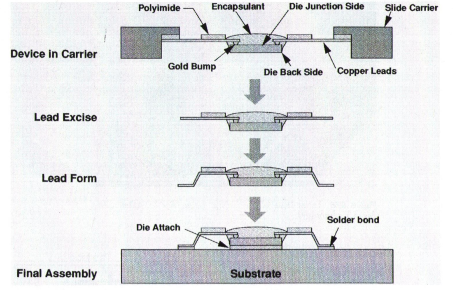
\includegraphics[scale=0.6]{images/TAB.png}
   \end{center}
   \caption{TAB}
\end{figure}

Rozvojem Flip Chip technologie a významným pokrokům v automatizaci WB přišla TAB
technologie o výsadní postavení ve Fine Pitch aplikacích. Komlikace také přináší návrh vývodů pro každý nový čip a rozložení vývodů. Také planarita na straně DPS či pouzdra je velmi důležitým faktorem. Výhodou zůstala možnost povádět elektrický test čipu nabo jeho zahoření před samotným připojením do obvodu nebo pouzdra.

\subsection{Flip Chip}
Jedná se o přímou metodu elektrického propojení a
mechanického připevnění čipu do obvodu či pouzdra.

Vzhledem k nutnosti vytvoření dostatečně velkých plošek u WB je možné u FC dosáhnout jedé z největší hustot integrace vývodového propojení.

Čip se umísťuje do obvodu aktivní plochou s vývody dolů (face down).

Bumpy mohou být připájeny nebo přilepeny pomocí vodivého lepidla - zvolená metoda
závisí na požadavcích spolehlivosti u dané aplikace.

Lepení FC pomocí vodivého epoxidového lepidla je levný, ale méně spolehlivý proces montáže. 

Anizotropní vodivé lepidlo slouží zároveň jako underfill.

\begin{figure}[h]
   \begin{center}
     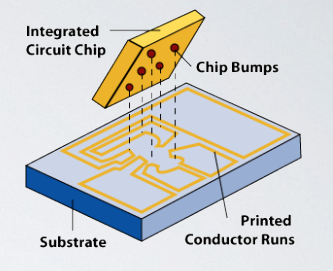
\includegraphics[scale=0.6]{images/FC.png}
   \end{center}
   \caption{Flip Chip}
\end{figure}

V případech, kdy je požadována vysoká spolehlivost, bývají používány především pájkové
bumpy, které se vytváří přímo na čipu.

Při montáži čipů na keramické substráty a pouzdra se nejčastěji používají bumpy s vyšší teplotou tavení. Důvodem je možné natavování během následné montáže na DPS.

Po připojení Flip Chipu se pro vylepšení mechanických vlastností a chemické odolnosti se nanáší na hrany FC epoxidové hmoty (underfills). Tyto zatékají díky kapilárnímu efektu do mezery mezi čipem a podložkou, kterou dokonale vyplní.

\begin{figure}[h]
   \begin{center}
     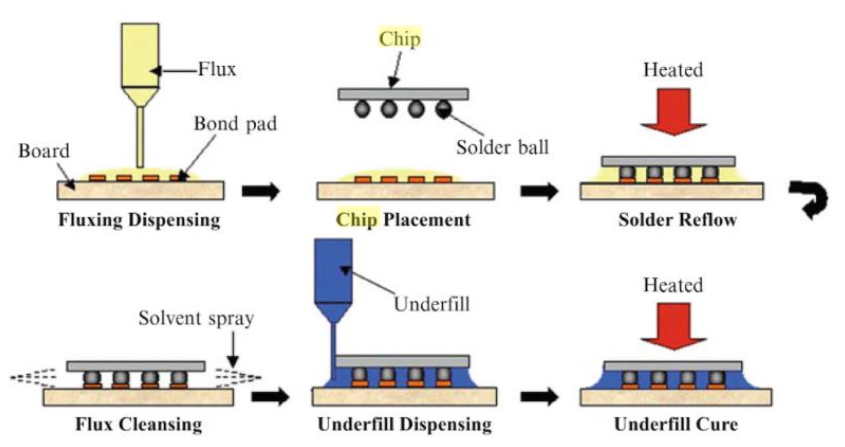
\includegraphics[scale=0.6]{images/FC2.png}
   \end{center}
   \caption{Flip Chip-underfills}
\end{figure}

Vzhledem k požadavku co nejlepšího souladu TCE křemíku, DPS a underfillu je nutné epoxidovou hmotu underfillu doplnit křemíkovým práškem, který TCE patřičně upraví.

Po připojení Flip Chipu se pro vylepšení mechanických vlastností a chemické odolnosti se nanáší na hrany FC epoxidové hmoty (underfills). Tyto zatékají díky kapilárnímu efektu do mezery mezi čipem a podložkou, kterou dokonale vyplní.

\subsection{Wire bonding}
Máme 3 základní typy:
\begin{itemize}
\item Ultrazvukové
\item Termokompresní
\item Termosonický
\end{itemize}

Bondování se dále rozděluje na:
\begin{itemize}
\item Hranové
\item Kuličkové
\end{itemize}

\subsubsection{Termokompresní}
\textbf{Termokompresní} sváření je jeden ze způsobů při kterém dochází k vytvoření sváru mezi mikrodrátkem a kontaktovací ploškou kombinací teploty a tlaku. Svár je vytvořen vzájemnou difůzí krystalové mřížky mikrodrátku a kontaktovací plošky. Teplota ohřevu kontaktovací plošky (250 $^{\circ}$C – 380 $^{\circ}$C) i mikrodrátku, který se od ní při kontaktování ohřívá je nižší než její teplota tavení a zbylá energie je dodána energií tlakovou. Používá se Au mikrodrátek o průměru 25 $\mu$m.

\subsubsection{Ultrazvukové}
\textbf{Ultrazvukové} sváření je realizováno intenzivním kmitavým pohybem (30
kHz - 120kHz), kdy dojde k přenosu ultrazvukové energie na rozhraní drátek - kontaktní ploška a nastává prolínání atomů mezi dvěma kovy (na základě smykového tření). Používá se zejména k připojení Al mikrodrátků na kontaktní plošky tenkých a tlustých kovových vrstev z Au, Ag, Ni nebo Pd. Spoj se vytváří při pokojové teplotě.
\begin{figure}[h]
   \begin{center}
     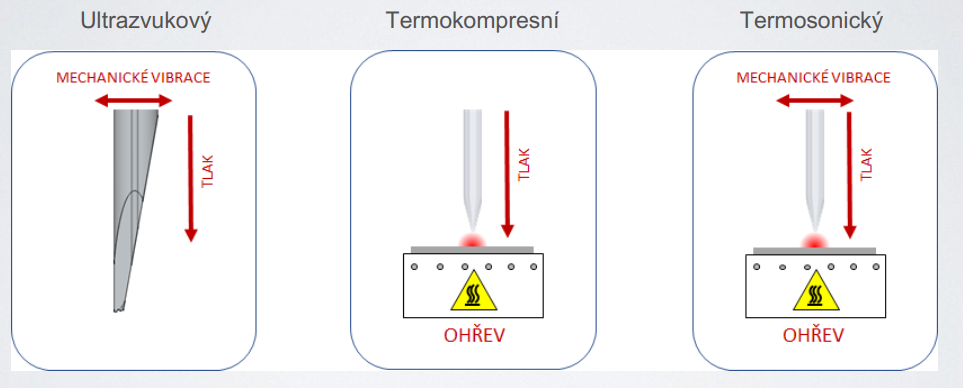
\includegraphics[scale=0.6]{images/Bond.png}
   \end{center}
   \caption{Rozdělení procesů}
\end{figure}

\subsubsection{Hranové bondování}
Zjednodušený postup wedge bondingu (kontaktování na hranu).

Využívá se difuze materiálu drátku do hmoty kontaktované plošky pomocí ultrazvukového kmitání (smykového tření).

Auto ball bonders jsou několikrát rychlejší než autowedge bonders. Důvodem je možnost posunu kapiláry (po prvním sváru) libovolným směrem.

U hranového kontaktování je nutné, aby byl drátek vzhledem ke kontaktovací kapiláře správně orientován.

Nástroj je vyroben obvykle z WC (v některých případech je z tohoto
materiálu pouze špička nástroje).

Vyskytují se také nástroje z dalších tvrdých materiálů, jakými je například TiC.
\begin{figure}[h]
   \begin{center}
     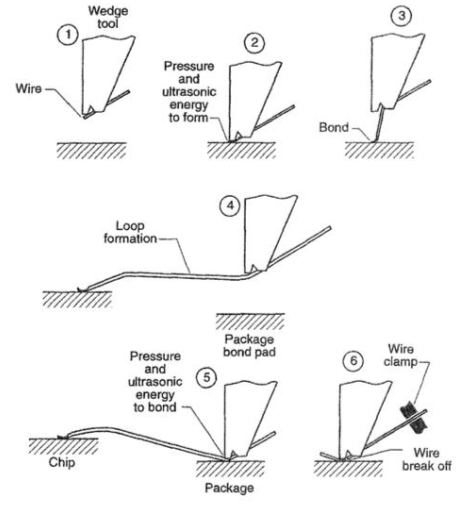
\includegraphics[scale=0.6]{images/Hrana.png}
   \end{center}
   \caption{WEDGE Bonding (Hranové)}
\end{figure}

\subsubsection{Kuličkové bondování}
Vytvoření kuličky elektrickým výbojem nebo plamínkem.

Umístění kapiláry nad plošku čipu.

Vytvoření prvního spoje za pomocí tlaku, tepla a UZ kmitání.

Formování smyčky (přesná sekvence řízených pohybů).

Umístění kapiláry nad plošku pouzdra nebo substrátu.

Vytvoření druhého spoje za pomocí tlaku, tepla a UZ kmitání.

Odtržení drátku.

Realizace dalšího propojení.

Používají se opět i další tvrdé materiály. Vyskytují je například safírové nebo rubínové špičky.

\begin{figure}[h]
   \begin{center}
     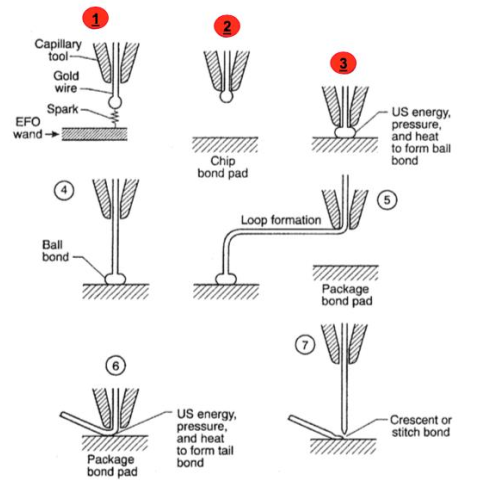
\includegraphics[scale=0.6]{images/Ball.png}
   \end{center}
   \caption{BALL Bonding (Kuličkové)}
\end{figure}

\subsubsection{Materiály pro wirebonding}
\textbf{Standardní mikrodátky z:} Au, Cu, AlSi\\
\textbf{Pro speciální aplikace z:} Ag, Pd, Au-Al, Pd-Cu













